\documentclass[../master/master.tex]{subfiles}
\begin{document}
Once the algorithms had been implemented, we needed to find some inputs to conduscct our experiments. We found large datasets
Small graphs:
\begin{itemize}
\item not so much correlation between nodes and steps
\item moderate positive correlation between nodes and time
\item moderate positive correlation between number of SCCs in graph and steps - although with some outliers if there are many nodes in an SCC
\item generally negative correaltion between how many nodes there are per scc and steps
\item linears and locksteps tend to stick together, with trimming helping slightly some of the time. Linears generally tend to do a little worse than locksteps
\item locksteps seem to perform better time wise, but worse step wise
\end{itemize}
Big graphs:
\begin{itemize}
\item slight positive correlation between nodes and steps if trimmign not used - trimming improves complexity
\item slight positive, but really no correlation between time and nodes, trimming improves runtime
\item positive correlation betwen no of SCCs and steps, trimming helps with bigger graphs
\item generally negative correlation between nodes per scc and steps, where trimming helps significantly on some data
\item linears perform slightly worse than locksteps in steps
\item linears are slightly better on larger datasets time-wise
\end{itemize}

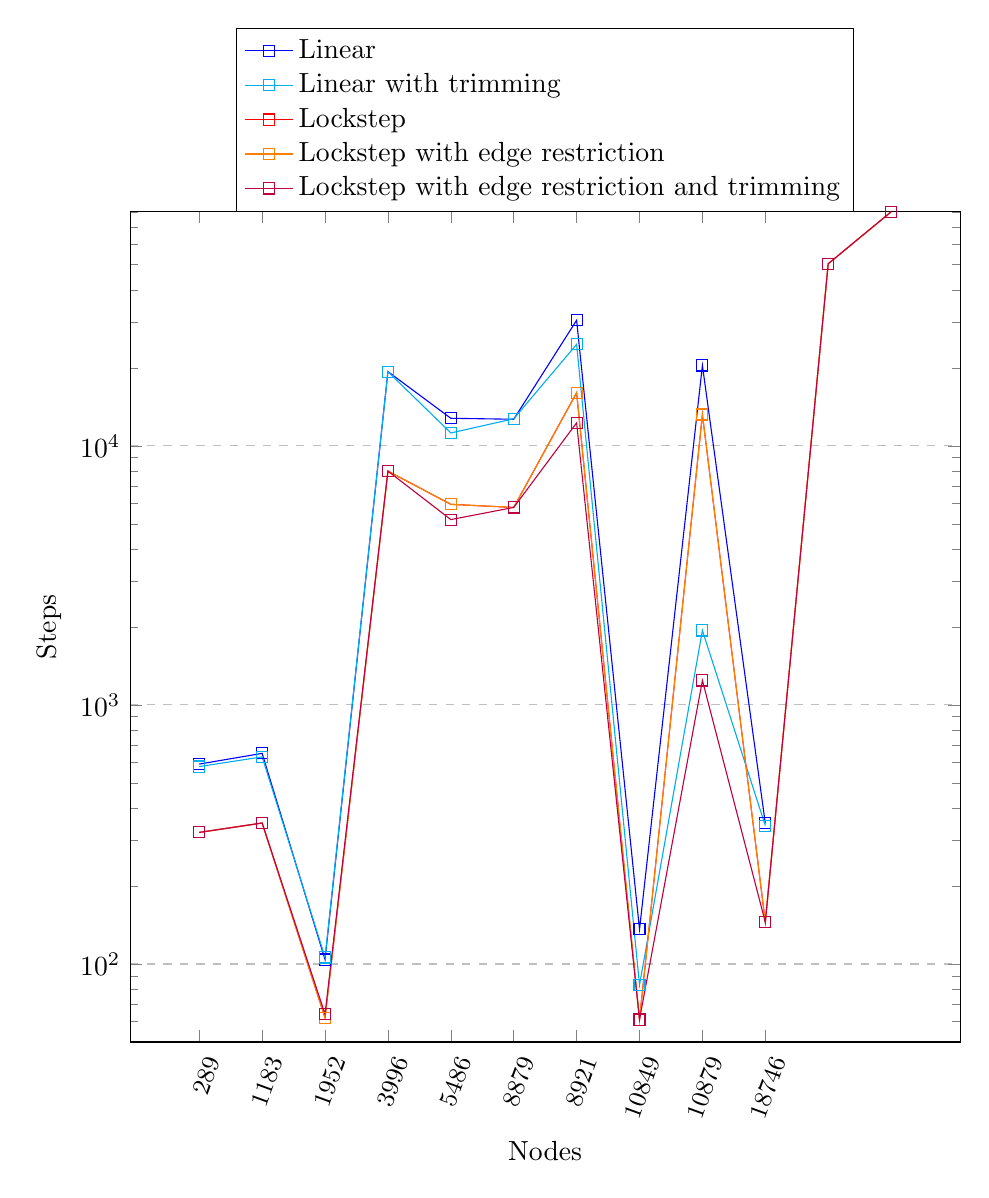
\begin{tikzpicture}
\begin{axis}[
height = \textwidth,
width=\textwidth,
xtick=data,
x tick label style = {font = \small, align = center, rotate = 70, anchor = north east},
title={Small graphs},
xlabel={Nodes},
ylabel={Steps},
ymin=50, ymax=80100,
legend style={at={(0.5,1)},anchor=south,legend cell align=left},
ymajorgrids=true,
grid style=dashed,
ymode=log,
log basis y={10},
symbolic x coords={289, 1183, 1952, 3996, 5486, 8879, 8921, 10849, 10879, 18746, 25217, 40006 }]
\addplot[color=blue,mark=square,]coordinates {(289, 591)(1183, 650)(1952, 104)(3996, 19344)(5486, 12773)(8879, 12664)(8921, 30529)(10849, 136)(10879, 20434)(18746, 349)(25217, 0)(40006, 0)};
\addplot[color=cyan,mark=square,]coordinates {(289, 578)(1183, 630)(1952, 106)(3996, 19332)(5486, 11211)(8879, 12716)(8921, 24640)(10849, 83)(10879, 1938)(18746, 342)(25217, 0)(40006, 0)};
\addplot[color=red,mark=square,]coordinates {(289, 322)(1183, 350)(1952, 62)(3996, 7992)(5486, 5945)(8879, 5783)(8921, 16032)(10849, 61)(10879, 13209)(18746, 145)(25217, 50434)(40006, 80011)};
\addplot[color=orange,mark=square,]coordinates {(289, 322)(1183, 350)(1952, 62)(3996, 7992)(5486, 5945)(8879, 5783)(8921, 16032)(10849, 61)(10879, 13209)(18746, 145)(25217, 50434)(40006, 80011)};
\addplot[color=purple,mark=square,]coordinates {(289, 322)(1183, 350)(1952, 64)(3996, 7990)(5486, 5191)(8879, 5783)(8921, 12264)(10849, 61)(10879, 1243)(18746, 145)(25217, 50432)(40006, 80013)};
\legend{Linear, Linear with trimming, Lockstep, Lockstep with edge restriction, Lockstep with edge restriction and trimming}
\end{axis}
\end{tikzpicture}

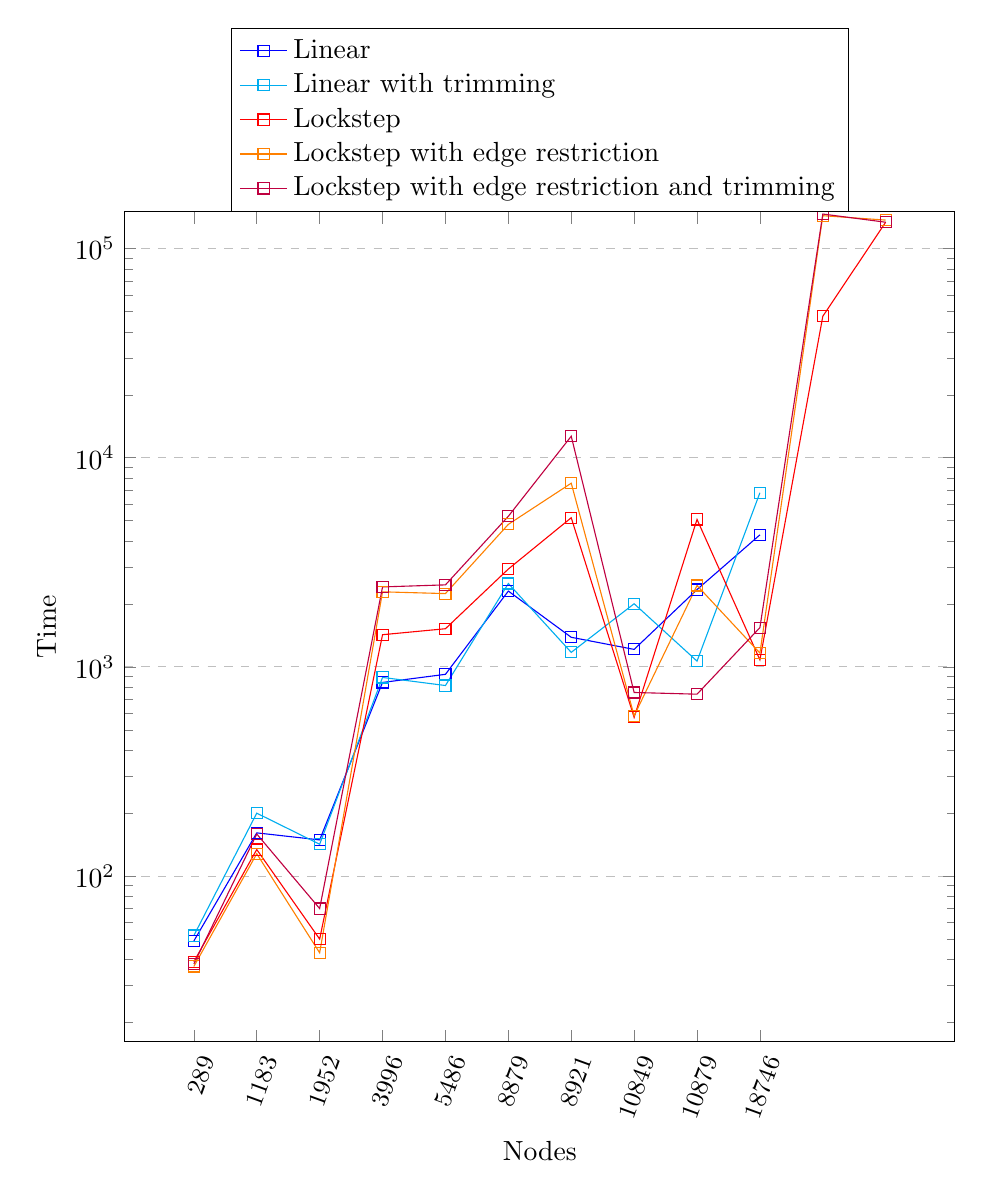
\begin{tikzpicture}
\begin{axis}[
height = \textwidth,
width=\textwidth,
xtick=data,
x tick label style = {font = \small, align = center, rotate = 70, anchor = north east},
title={Small graphs},
xlabel={Nodes},
ylabel={Time},
ymin=0, ymax=150000,
legend style={at={(0.5,1)},anchor=south,legend cell align=left},
ymajorgrids=true,
grid style=dashed,
ymode=log,
log basis y={10},
symbolic x coords={289, 1183, 1952, 3996, 5486, 8879, 8921, 10849, 10879, 18746, 25217, 40006 }]
\addplot[color=blue,mark=square,]coordinates {(289, 49)(1183, 161)(1952, 149)(3996, 843)(5486, 922)(8879, 2305)(8921, 1386)(10849, 1213)(10879, 2343)(18746, 4279)(25217, 0)(40006, 0)};
\addplot[color=cyan,mark=square,]coordinates {(289, 52)(1183, 200)(1952, 142)(3996, 891)(5486, 815)(8879, 2505)(8921, 1174)(10849, 2005)(10879, 1066)(18746, 6804)(25217, 0)(40006, 0)};
\addplot[color=red,mark=square,]coordinates {(289, 39)(1183, 134)(1952, 50)(3996, 1426)(5486, 1523)(8879, 2938)(8921, 5167)(10849, 574)(10879, 5072)(18746, 1081)(25217, 47465)(40006, 133708)};
\addplot[color=orange,mark=square,]coordinates {(289, 37)(1183, 128)(1952, 43)(3996, 2286)(5486, 2242)(8879, 4804)(8921, 7558)(10849, 584)(10879, 2451)(18746, 1165)(25217, 143599)(40006, 136794)};
\addplot[color=purple,mark=square,]coordinates {(289, 38)(1183, 159)(1952, 70)(3996, 2413)(5486, 2468)(8879, 5250)(8921, 12674)(10849, 755)(10879, 741)(18746, 1542)(25217, 146235)(40006, 133621)};
\legend{Linear, Linear with trimming, Lockstep, Lockstep with edge restriction, Lockstep with edge restriction and trimming}
\end{axis}
\end{tikzpicture}

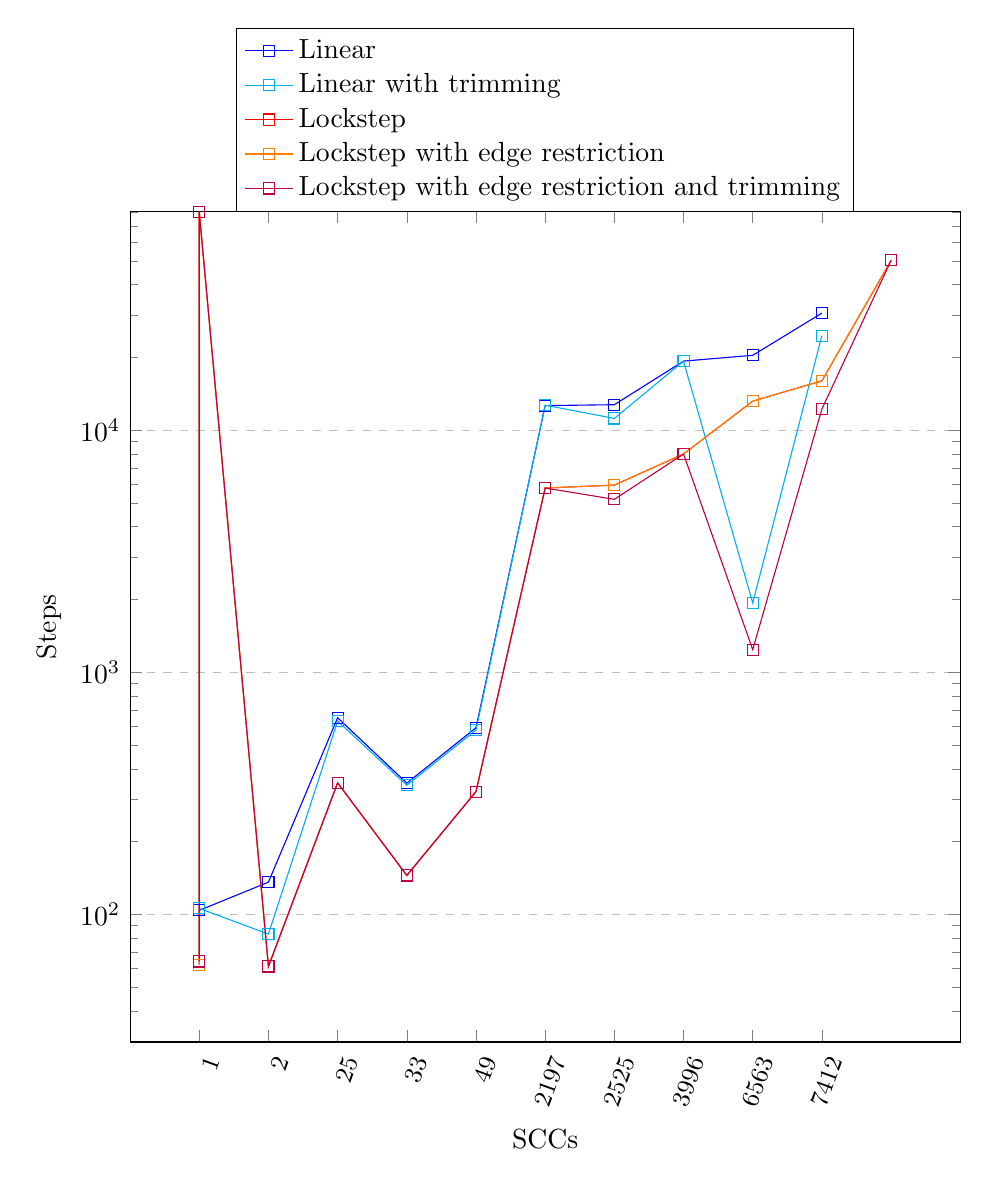
\begin{tikzpicture}
\begin{axis}[
height = \textwidth,
width=\textwidth,
xtick=data,
x tick label style = {font = \small, align = center, rotate = 70, anchor = north east},
title={Small graphs},
xlabel={SCCs},
ylabel={Steps},
ymin=0, ymax=80100,
legend style={at={(0.5,1)},anchor=south,legend cell align=left},
ymajorgrids=true,
grid style=dashed,
ymode=log,
log basis y={10},
symbolic x coords={0, 0, 1, 2, 25, 33, 49, 2197, 2525, 3996, 6563, 7412, 25217 }]
\addplot[color=blue,mark=square,]coordinates {(1, 104)(1, 0)(2, 136)(25, 650)(33, 349)(49, 591)(2197, 12664)(2525, 12773)(3996, 19344)(6563, 20434)(7412, 30529)(25217, 0)};
\addplot[color=cyan,mark=square,]coordinates {(1, 106)(1, 0)(2, 83)(25, 630)(33, 342)(49, 578)(2197, 12716)(2525, 11211)(3996, 19332)(6563, 1938)(7412, 24640)(25217, 0)};
\addplot[color=red,mark=square,]coordinates {(1, 62)(1, 80011)(2, 61)(25, 350)(33, 145)(49, 322)(2197, 5783)(2525, 5945)(3996, 7992)(6563, 13209)(7412, 16032)(25217, 50434)};
\addplot[color=orange,mark=square,]coordinates {(1, 62)(1, 80011)(2, 61)(25, 350)(33, 145)(49, 322)(2197, 5783)(2525, 5945)(3996, 7992)(6563, 13209)(7412, 16032)(25217, 50434)};
\addplot[color=purple,mark=square,]coordinates {(1, 64)(1, 80013)(2, 61)(25, 350)(33, 145)(49, 322)(2197, 5783)(2525, 5191)(3996, 7990)(6563, 1243)(7412, 12264)(25217, 50432)};
\legend{Linear, Linear with trimming, Lockstep, Lockstep with edge restriction, Lockstep with edge restriction and trimming}
\end{axis}
\end{tikzpicture}

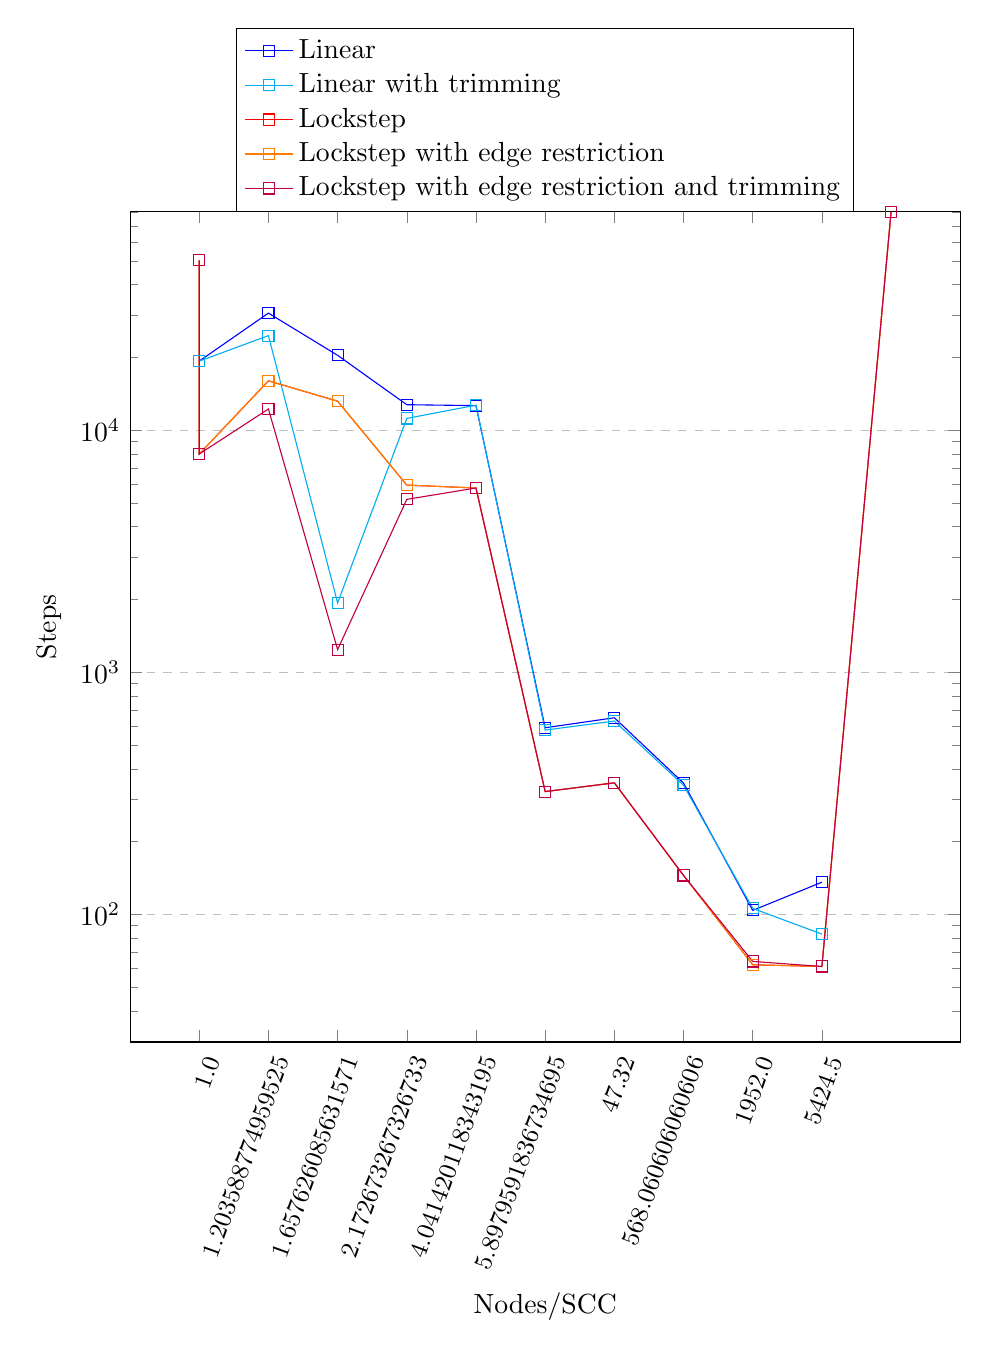
\begin{tikzpicture}
\begin{axis}[
height = \textwidth,
width=\textwidth,
xtick=data,
x tick label style = {font = \small, align = center, rotate = 70, anchor = north east},
title={Small graphs},
xlabel={Nodes/SCC},
ylabel={Steps},
ymin=0, ymax=80100,
legend style={at={(0.5,1)},anchor=south,legend cell align=left},
ymajorgrids=true,
grid style=dashed,
ymode=log,
log basis y={10},
symbolic x coords={ 1.0, 1.0, 1.203588774959525, 1.657626085631571, 2.172673267326733, 4.041420118343195, 5.8979591836734695, 47.32, 568.060606060606, 1952.0, 5424.5, 40006.0}]
\addplot[color=blue,mark=square,]coordinates {(1.0, 0)(1.0, 19344)(1.203588774959525, 30529)(1.657626085631571, 20434)(2.172673267326733, 12773)(4.041420118343195, 12664)(5.8979591836734695, 591)(47.32, 650)(568.060606060606, 349)(1952.0, 104)(5424.5, 136)(40006.0, 0)};
\addplot[color=cyan,mark=square,]coordinates {(1.0, 0)(1.0, 19332)(1.203588774959525, 24640)(1.657626085631571, 1938)(2.172673267326733, 11211)(4.041420118343195, 12716)(5.8979591836734695, 578)(47.32, 630)(568.060606060606, 342)(1952.0, 106)(5424.5, 83)(40006.0, 0)};
\addplot[color=red,mark=square,]coordinates {(1.0, 50434)(1.0, 7992)(1.203588774959525, 16032)(1.657626085631571, 13209)(2.172673267326733, 5945)(4.041420118343195, 5783)(5.8979591836734695, 322)(47.32, 350)(568.060606060606, 145)(1952.0, 62)(5424.5, 61)(40006.0, 80011)};
\addplot[color=orange,mark=square,]coordinates {(1.0, 50434)(1.0, 7992)(1.203588774959525, 16032)(1.657626085631571, 13209)(2.172673267326733, 5945)(4.041420118343195, 5783)(5.8979591836734695, 322)(47.32, 350)(568.060606060606, 145)(1952.0, 62)(5424.5, 61)(40006.0, 80011)};
\addplot[color=purple,mark=square,]coordinates {(1.0, 50432)(1.0, 7990)(1.203588774959525, 12264)(1.657626085631571, 1243)(2.172673267326733, 5191)(4.041420118343195, 5783)(5.8979591836734695, 322)(47.32, 350)(568.060606060606, 145)(1952.0, 64)(5424.5, 61)(40006.0, 80013)};
\legend{Linear, Linear with trimming, Lockstep, Lockstep with edge restriction, Lockstep with edge restriction and trimming}
\end{axis}
\end{tikzpicture}

\begin{tikzpicture}
\begin{axis}[
height = \textheight,
width=\textwidth,
xtick=data,
x tick label style = {font = \small, align = center, rotate = 70, anchor = north east},
title={Big graphs},
xlabel={Nodes},
ylabel={Steps},
ymin=0, ymax=3000000,
legend style={at={(0.5,1)},anchor=south,legend cell align=left},
ymajorgrids=true,
grid style=dashed,
ymode=log,
log basis y={10},
symbolic x coords={52268, 83436, 116456, 157604, 281903, 720247}]
\addplot[color=blue,mark=square,]coordinates {(52268, 48495)(83436, 1661)(116456, 560414)(157604, 570525)(281903, 0)(720247, 2156545)};
\addplot[color=cyan,mark=square,]coordinates {(52268, 48497)(83436, 1658)(116456, 560411)(157604, 344348)(281903, 0)(720247, 20945)};
\addplot[color=red,mark=square,]coordinates {(52268, 30384)(83436, 986)(116456, 0)(157604, 291672)(281903, 0)(720247, 1435356)};
\addplot[color=orange,mark=square,]coordinates {(52268, 30384)(83436, 986)(116456, 0)(157604, 0)(281903, 122371)(720247, 1435356)};
\addplot[color=purple,mark=square,]coordinates {(52268, 30386)(83436, 986)(116456, 0)(157604, 169828)(281903, 81275)(720247, 13872)};
\legend{Linear, Linear with trimming, Lockstep, Lockstep with edge restriction, Lockstep with edge restriction and trimming}
\end{axis}
\end{tikzpicture}

\begin{tikzpicture}
\begin{axis}[
height = \textheight,
width=\textwidth,
xtick=data,
x tick label style = {font = \small, align = center, rotate = 70, anchor = north east},
title={Small graphs},
xlabel={Nodes},
ylabel={Time},
ymin=0, ymax=1600000,
legend style={at={(0.5,1)},anchor=south,legend cell align=left},
ymajorgrids=true,
grid style=dashed,
ymode=log,
log basis y={10},
symbolic x coords={52268, 83436, 116456, 157604, 281903, 720247 }]
\addplot[color=blue,mark=square,]coordinates {(52268, 25608)(83436, 13562)(116456, 146786)(157604, 253563)(281903, 0)(720247, 97531)};
\addplot[color=cyan,mark=square,]coordinates {(52268, 27534)(83436, 15691)(116456, 149855)(157604, 191313)(281903, 0)(720247, 23638)};
\addplot[color=red,mark=square,]coordinates {(52268, 117469)(83436, 9936)(116456, 0)(157604, 1542037)(281903, 0)(720247, 732579)};
\addplot[color=orange,mark=square,]coordinates {(52268, 23209)(83436, 4034)(116456, 0)(157604, 0)(281903, 1216873)(720247, 159329)};
\addplot[color=purple,mark=square,]coordinates {(52268, 25463)(83436, 6205)(116456, 0)(157604, 1137648)(281903, 834071)(720247, 47275)};
\legend{Linear, Linear with trimming, Lockstep, Lockstep with edge restriction, Lockstep with edge restriction and trimming}
\end{axis}
\end{tikzpicture}

\begin{tikzpicture}
\begin{axis}[
height = \textheight,
width=\textwidth,
xtick=data,
x tick label style = {font = \small, align = center, rotate = 70, anchor = north east},
title={Small graphs},
xlabel={SCCs},
ylabel={Steps},
ymin=0, ymax=3000000,
legend style={at={(0.5,1)},anchor=south,legend cell align=left},
ymajorgrids=true,
grid style=dashed,
ymode=log,
log basis y={10},
symbolic x coords={0, 253, 11828, 29914, 116456, 143111, 713126 }]
\addplot[color=blue,mark=square,]coordinates {(253, 1661)(11828, 48495)(29914, 0)(116456, 560414)(143111, 570525)(713126, 2156545)};
\addplot[color=cyan,mark=square,]coordinates {(253, 1658)(11828, 48497)(29914, 0)(116456, 560411)(143111, 344348)(713126, 20945)};
\addplot[color=red,mark=square,]coordinates {(253, 986)(11828, 30384)(29914, 0)(116456, 0)(143111, 291672)(713126, 1435356)};
\addplot[color=orange,mark=square,]coordinates {(253, 986)(11828, 30384)(29914, 122371)(116456, 0)(143111, 291672)(713126, 1435356)};
\addplot[color=purple,mark=square,]coordinates {(253, 986)(11828, 30386)(29914, 81275)(116456, 0)(143111, 169828)(713126, 13872)};
\legend{Linear, Linear with trimming, Lockstep, Lockstep with edge restriction, Lockstep with edge restriction and trimming}
\end{axis}
\end{tikzpicture}

\begin{tikzpicture}
\begin{axis}[
height = \textheight,
width=\textwidth,
xtick=data,
x tick label style = {font = \small, align = center, rotate = 70, anchor = north east},
title={Small graphs},
xlabel={Nodes/SCC},
ylabel={Steps},
ymin=0, ymax=3000000,
legend style={at={(0.5,1)},anchor=south,legend cell align=left},
ymajorgrids=true,
grid style=dashed,
ymode=log,
log basis y={10},
symbolic x coords={1.0, 1.0099856126406834, 1.1012710413595042, 4.419005749070004, 9.423781506986694, 329.7865612648221 }]
\addplot[color=blue,mark=square,]coordinates {(1.0, 560414)(1.0099856126406834, 2156545)(1.1012710413595042, 570525)(4.419005749070004, 48495)(9.423781506986694, 0)(329.7865612648221, 1661)};
\addplot[color=cyan,mark=square,]coordinates {(1.0, 560411)(1.0099856126406834, 20945)(1.1012710413595042, 344348)(4.419005749070004, 48497)(9.423781506986694, 0)(329.7865612648221, 1658)};
\addplot[color=red,mark=square,]coordinates {(1.0, 0)(1.0099856126406834, 1435356)(1.1012710413595042, 291672)(4.419005749070004, 30384)(9.423781506986694, 0)(329.7865612648221, 986)};
\addplot[color=orange,mark=square,]coordinates {(1.0, 0)(1.0099856126406834, 1435356)(4.419005749070004, 30384)(9.423781506986694, 122371)(9.423781506986694, 0)(329.7865612648221, 986)};
\addplot[color=purple,mark=square,]coordinates {(1.0, 0)(1.0099856126406834, 13872)(1.1012710413595042, 169828)(4.419005749070004, 30386)(9.423781506986694, 81275)(329.7865612648221, 986)};
\legend{Linear, Linear with trimming, Lockstep, Lockstep with edge restriction, Lockstep with edge restriction and trimming}
\end{axis}
\end{tikzpicture}

\end{document}
%%% Local Variables:
%%% mode: latex
%%% TeX-master: "../master/master"
%%% End:
